\documentclass[letterpaper,10pt]{article}
\title{Winter Progress Report for RockSat-X Payload - Hephaestus \\ Group 26}
\author{Amber~Horvath\\ \\ CS462 - Winter 2017}
\usepackage[pdftex]{graphicx}
\usepackage{tikz}
\usepackage{float}

\parindent = 0.0 in
\parskip = 0.1 in

\begin{document}
\maketitle

\section{Introduction}
The Hephaestus Payload is a rocketry payload that will fly onboard the 2016-2017 RockSat-X rocket. 
The rocket will be launched from the Wallops Flight Facility filled with student-made payloads from 
various institutions. The Hephaestus payload will consist of a deployable arm and a video camera.
The arm shall extend and move to a series of pre-placed sensors and make contact with the sensors. 
The arm will then contract and retract back into the rocket.
The video camera shall record the arm's movement. Data about the flight, such as error codes, shall be 
sent via a telemetry port and written onto a microSD card.
The Hephaestus mission will be Oregon State University's first space mission and will prove not only
our ability to develop a space-ready payload, but also the viability of construction in space using a robotic
arm.
\section{Individual Pieces}
The individual pieces of the project I am in charge of for the project include Emergency Retraction, 
Modes of Operation, and Touch Sensor Viability. I also took on the Data Storage task by the request
of the Electrical Engineering team.
\subsection{Emergency Retraction}
In the case of the arm getting caught in a bad state, we shall retract the arm back into a safe state
This will be accomplished by testing for a bad state.
We will retract the arm and test whether or not we?re in our calibrated normal position
If we are not, we are in a bad state and need to execute the emergency arm retraction.
We will then disable each motor except the one attached to the base of the payload.
Once each motor has been disabled, we will retract the base of the payload.
\subsection{Modes of Operation}

\begin{center}
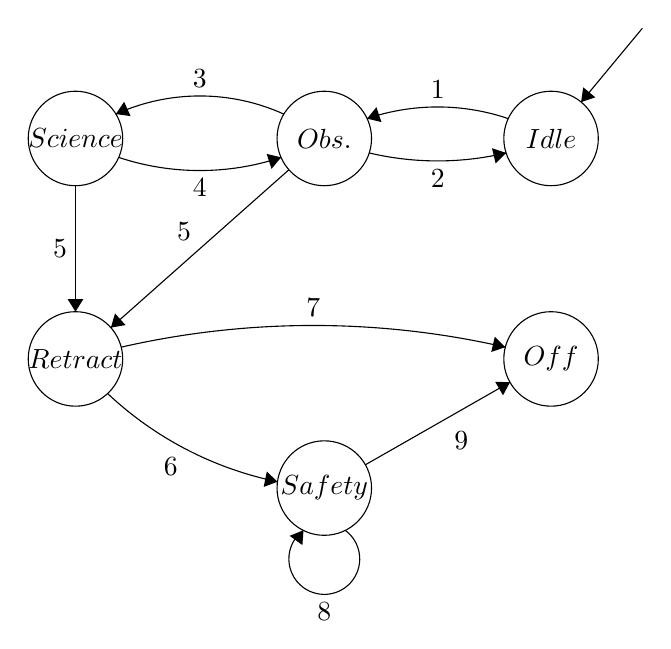
\begin{tikzpicture}[scale=0.2]
\tikzstyle{every node}+=[inner sep=0pt]
\draw [black] (46.2,-13.5) circle (3);
\draw (46.2,-13.5) node {$Idle$};
\draw [black] (31.8,-13.5) circle (3);
\draw (31.8,-13.5) node {$Obs.$};
\draw [black] (16,-13.5) circle (3);
\draw (16,-13.5) node {$Science$};
\draw [black] (16,-27.5) circle (3);
\draw (16,-27.5) node {$Retract$};
\draw [black] (46.2,-27.5) circle (3);
\draw (46.2,-27.5) node {$Off$};
\draw [black] (31.8,-35.7) circle (3);
\draw (31.8,-35.7) node {$Safety$};
\draw [black] (52,-6.5) -- (48.11,-11.19);
\fill [black] (48.11,-11.19) -- (49.01,-10.89) -- (48.24,-10.25);
\draw [black] (34.516,-12.239) arc (108.749:71.251:13.951);
\fill [black] (34.52,-12.24) -- (35.43,-12.46) -- (35.11,-11.51);
\draw (39,-11) node [above] {$1$};
\draw [black] (43.348,-14.419) arc (-76.68931:-103.31069:18.884);
\fill [black] (43.35,-14.42) -- (42.45,-14.12) -- (42.68,-15.09);
\draw (39,-15.43) node [below] {$2$};
\draw [black] (18.564,-11.955) arc (114.4174:65.5826:12.909);
\fill [black] (18.56,-11.95) -- (19.5,-12.08) -- (19.09,-11.17);
\draw (23.9,-10.3) node [above] {$3$};
\draw [black] (29.056,-14.702) arc (-71.60296:-108.39704:16.337);
\fill [black] (29.06,-14.7) -- (28.14,-14.48) -- (28.45,-15.43);
\draw (23.9,-16.04) node [below] {$4$};
\draw [black] (16,-16.5) -- (16,-24.5);
\fill [black] (16,-24.5) -- (16.5,-23.7) -- (15.5,-23.7);
\draw (15.5,-20.5) node [left] {$5$};
\draw [black] (29.55,-15.49) -- (18.25,-25.51);
\fill [black] (18.25,-25.51) -- (19.18,-25.35) -- (18.51,-24.61);
\draw (22.89,-20.01) node [above] {$5$};
\draw [black] (28.83,-35.296) arc (-101.59962:-133.25786:22.283);
\fill [black] (28.83,-35.3) -- (28.15,-34.65) -- (27.95,-35.63);
\draw (22.05,-33.75) node [below] {$6$};
\draw [black] (34.41,-34.22) -- (43.59,-28.98);
\fill [black] (43.59,-28.98) -- (42.65,-28.95) -- (43.15,-29.81);
\draw (40.5,-32.1) node [below] {$9$};
\draw [black] (33.123,-38.38) arc (54:-234:2.25);
\draw (31.8,-42.95) node [below] {$8$};
\fill [black] (30.48,-38.38) -- (29.6,-38.73) -- (30.41,-39.32);
\draw [black] (18.905,-26.751) arc (102.88102:77.11898:54.705);
\fill [black] (43.3,-26.75) -- (42.63,-26.09) -- (42.4,-27.06);
\draw (31.1,-24.87) node [above] {$7$};


\end{tikzpicture}
\end{center}



The Modes of Operation detail the states the program will be in during the course of the flight, as seen in the included state diagram. The transitions are as such:
\begin{enumerate}
\item{\textbf{Apogee is reached.} The experiment begins; the camera is powered on; and the on-board 
computer is on. A camera sweep is performed.}
\item{\textbf{Error: Return to Idle.} If an error occurs, we shall transition back to Idle mode.}
\item{\textbf{Payload Assembly and Camera have been deployed.} The software shall enter Science
mode once the payload assembly has been deployed and the camera sweep has completed.}
\item{\textbf{Error: Return to Observation.} If an error occurs, we transition back to Observation mode.}
\item{\textbf{Timer switch to end apogee period.} Experiment time has ended, proceed to Retract mode 
to prepare for descent.}
 \item{\textbf{Error: Proceed to Safety.} If the arm fails to retract, proceed to Safety mode.}
 \item{\textbf{Power off.} Arm is retracted, payload is retracted, computer is powered off, camera is 
 powered off. Payload is ready for descent.}
 \item{\textbf{Cycle in Safety.} Continually attempt to retract the arm and payload and power off the 
 computer and camera.}
 \item{\textbf{Power off.} Payload is now ready for descent.}
\end{enumerate}
\subsection{Touch Sensor Viability}
Within the body of the payload, two touch sensors will be placed at predetermined locations.
The arm shall make contact with the touch sensor and press it.
Upon being pressed, the touch sensor will go high and send a signal over telemetry and be written to
an SD card. The arm will then recalibrate before moving to the next sensor. If no sensors remain, 
the arm will retract and await shutdown.

\section{Progress and Problems}
\subsection{Emergency Retraction}
Due to the testing of emergency retraction being dependent upon the payload being assembled and the 
motors being attached to the payload, this has been a lower priority task. Pseudocode was written that 
details how this component of the project interacts with the other components of the program, but the 
code has not yet been completed. Code has been written for the interrupt subroutine that will notify the 
on-board computer to halt the current process and power off the specified motors.
\subsection{Modes of Operation}
The Modes of Operation requirement was technically completed last term, as it was essentially a state 
diagram that detailed how the program would operate throughout the flight. A state was added during the 
middle of the term to account for the time when the payload is being retracted from its extended state, 
but no other changes were made. As more code is being written, the modes of operation requirement will 
entail me ensuring that the design of the program upholds the design we originally developed last term.
\subsection{Touch Sensor Viability}
Similar to the Emergency Retraction requirement, due to dependencies of other components of the 
payload being assembled first, the Touch Sensor Viability requirement has been a lower-priority task. 
The dependences that must be resolved include determining the locations the arm will move to and 
implementing the code to move the arm to that location. Both those requirements are to be completed by 
Helena and her sub-team, "Pathing and Automation".
\subsection{Data Storage}
The Data Storage requirement has been the requirement that I have worked on the most the past term.
This is due to the other requirements having dependencies that must be resolved before progress
can be made, and the Electrical Engineers wanting this to be completed. The Data Storage component of the overall project has included numerous steps for completion including researching previous projects
similar to ours that required a micro controller and SD card, researching how SD cards work, requesting
assistance from experts around campus, and implementing the code and writing code specific to our ATMega128 and micoSD card. After researching solutions already in place for the larger question our team had ("How can you write data to an SD card from an ATMega128 micro controller?"), we chose to 
leverage the already-existing FatFS library, written by Elm-chan. The code is written in C and includes
a variety of files, some of which required ATMega128-specific code to be added in order to make it
compile and run. 

\begin{figure}[H]
\begin{center}
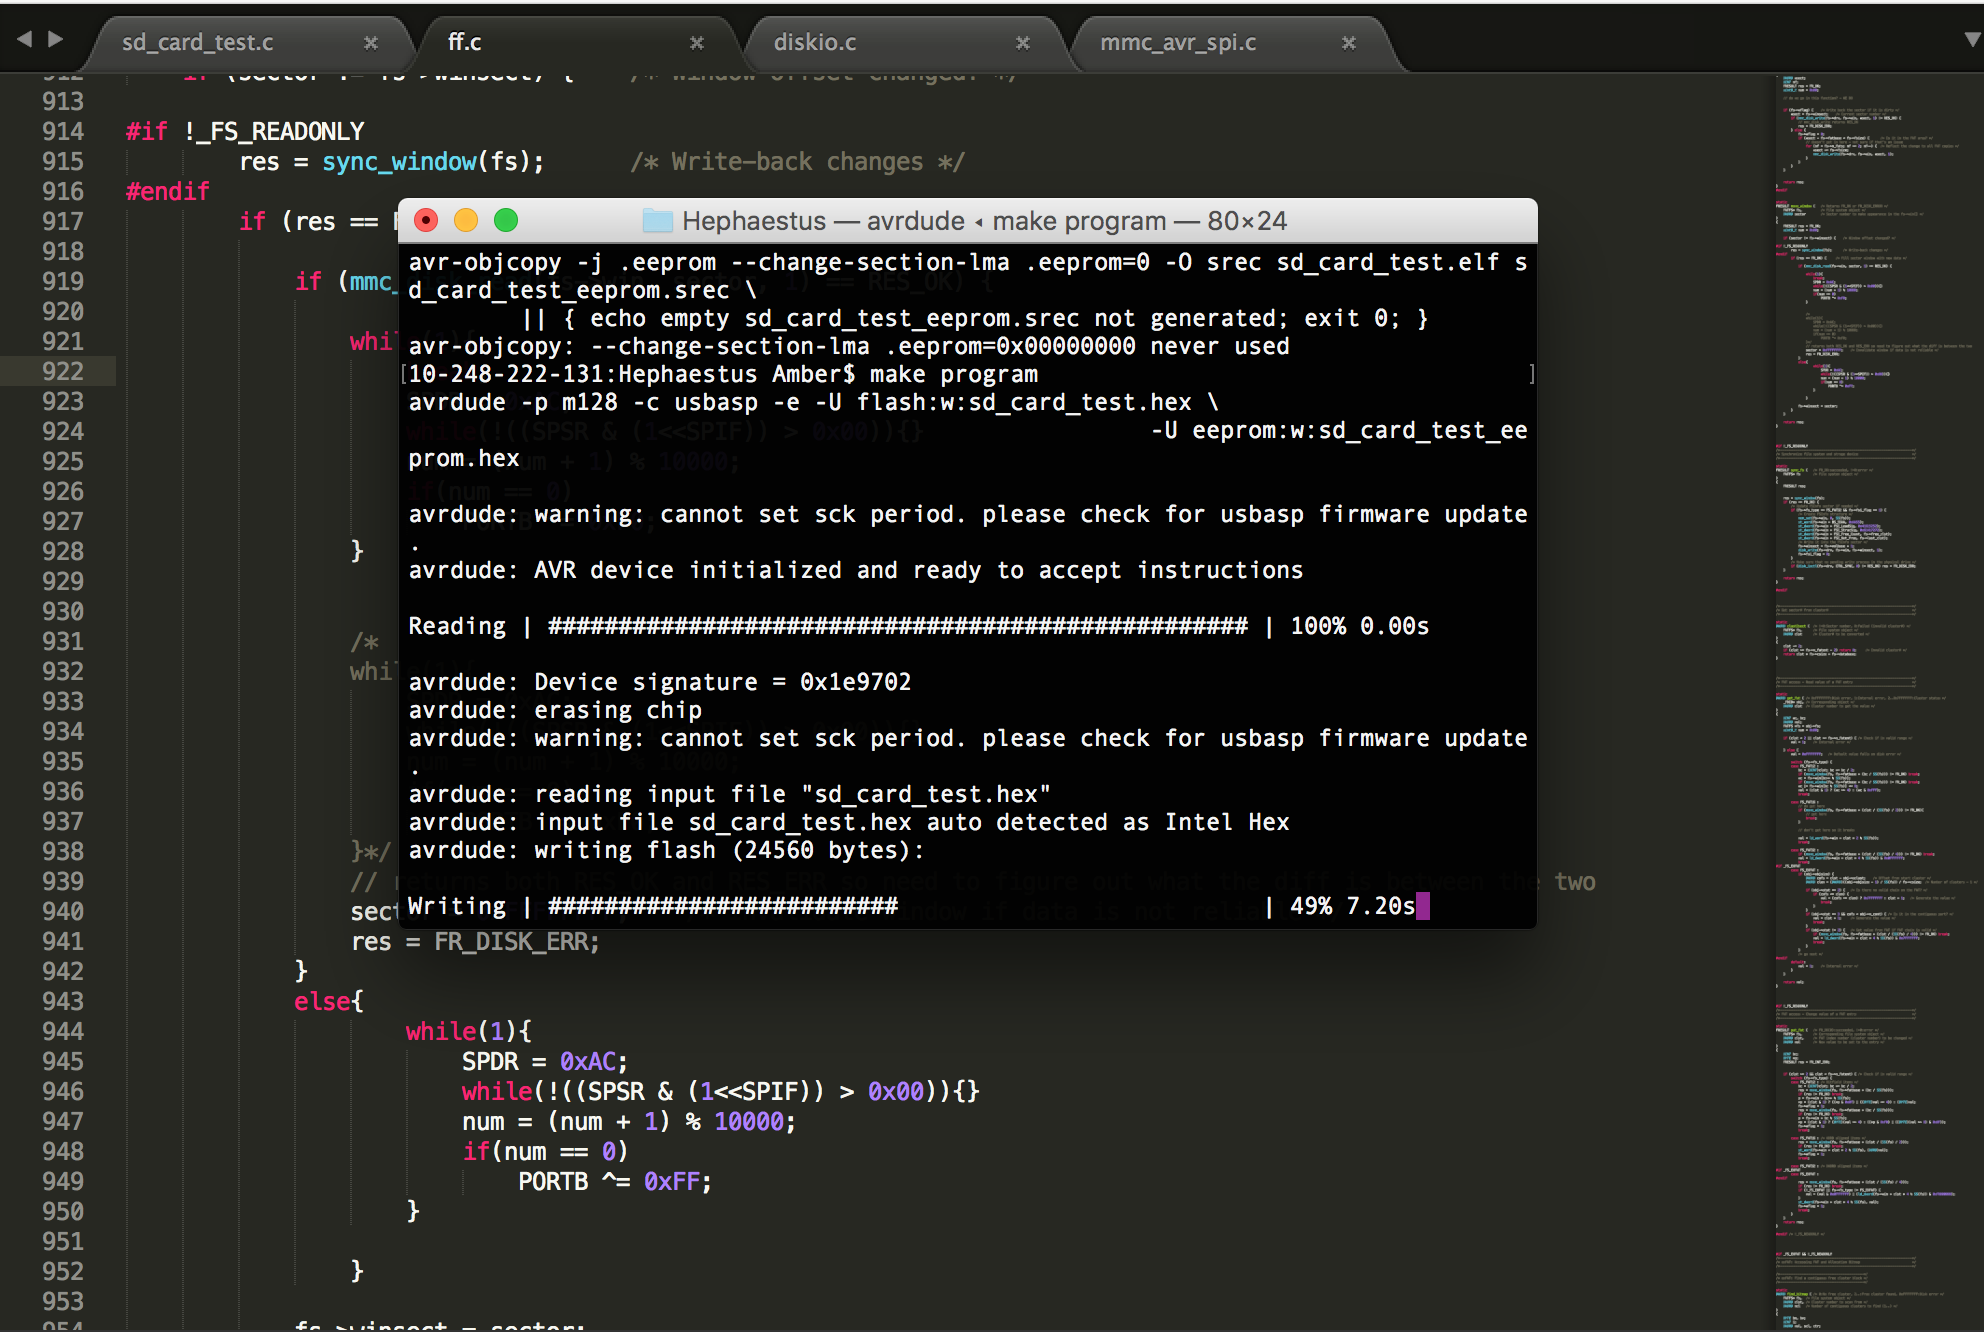
\includegraphics[height=5cm,width=\linewidth,keepaspectratio]{code.png}
\caption{An editor showing the files primarily used from the FatFS library and the code compiling with the avrdude compiler}
\label{fig:code}
\end{center}
\end{figure}
As shown in Figure \ref{fig:code}, there are 4 files currently open in the editor. One is "sdcardtest.c", 
which is the current file being used to test the core functionality our system requires. Our system must 
be able to open a file, write or append some data to the opened file, and close the file. 
These functionalities map to the API calls specified in "ff.c", the currently open file in Figure 
\ref{fig:code}. The main focus of my effort has been on getting these API calls to work as we intend
for them to. Currently, calls to the "fmount" function, which mounts the filesystem onto the micro
controller, and the "fopen" function, which creates a file pointer, work. However, we have not
been able to get writing to a file to work. This has been a large blocker for progress as the errors thrown
are difficult to follow and, as evident within Figure \ref{fig:code} there is a large amount of code that
must be sifted through, with many function calls leading to other parts of the library. Another layer
of complexity comes from the specificity of the problem, as there is documentation and forum
posts about using the FatFS library, but few that are as specific as using an ATMega128 with
a microSD card of our specific type.


\section{Evaluation}
Our team has had ups and downs this term. During the beginning of the term, we did not have a clearly
established workflow and felt minimal to no progress was being made, which caused a lot of stress
between all of us. Fortunately, we have put in systems such as mandatory group meetings and a scrum
update worksheet so we can ensure progress is being made. I believe our team will be a successful
development team as long as we continue adhering to these practices.
\subsection{Amber Horvath}
My main area of contribution has been on the Data Storage component as previously described.
I have put a lot of time and effort into this component and have collaborated with my peers,
namely Michael and our Electrical Engineer, Jonathan Hardman. I have also collaborated
with professors that are experts in this domain such as Roger Traylor. I am satisfied with the 
contribution to this team I've made over the course of the term. While I would've liked to
have the SD Card component fully completed by the end of this term, due to the nature of the
problem and the amount of work that is required to debug the program, I am trying to not be too hard on
 myself for not finishing this component. As for my role on the team, I feel I have fulfilled the duty of 
 keeping communication consistent and alive between team members. I have also tried to be a positive
 and empathetic member of the team so if spirits are getting low I try to get them back up. I feel
 the amount of work I have done is roughly equal to or above the other two members. This
 should be evident based on the blog post updates. However, it is hard to judge as a lot of our
 work has been collaborative and thus spread mainly evenly.
 \subsection{Helena Bales}
 Helena has filled the role of keeping the team focused and having the most expertise in the work
 we're doing. Due to her previous experience working with NASA and the UG Small Sat Lab, she
 is knowledgeable on more of the components of the project then myself. Overall, Helena's contribution
 to the team is probably lower or equal to myself and Michael's contribution. She was pivotal in the
 past couple weeks by mapping the Configuration Space and collaborating with the Pathing and
 Automation sub-team on that work, but it was harder to see progress being made prior to that point
 in the project. This is something our team could work on - having better communication between team
 members on progress or why progress is unable to occur.
 \subsection{Michael Humphrey}
 Michael has filled the role of keeping our information organized as he has been tasked with submitting
 group assignments. Michael has shown a commitment to staying on top of his workload and his
 level of organization has been an important asset to the team. I feel Michael's contribution to the
 project has been equivalent or less than mine. Michael worked on the Telemetry and Data Visualization
 component this term and showed progress, but not a largely significant amount. However, he did
 volunteer to help the Electrical Engineers and Mechanical Engineers on a testing component for their
 capstone classes which showed initiative that I appreciated. Overall, like Helena, I feel, due to the 
 nature of our project, towards the end of the term it was easier to see that he was making progress
 on his components of the project, but it would've been nice to know progress was being made
 all term.
 
\section{Retrospective}
\begin{center}
\begin{tabular}
%{ \textwidth }
{ | p{0.3\linewidth} | p{0.3\linewidth} | p{0.3\linewidth} | }
\hline
\textbf{Positives} & \textbf{Negatives} & \textbf{Changes} \\ \hline

We communicated with the larger team by holding weekly meetings. One person per team is required to represent the group at these meetings. & We did not take advantage of only one team member being required to attend the all-team meetings and usually had all three of our team members there. & We could change to usually only having two members attending, or not. \\ \hline

	We have established cross-functional team meetings. There are three cross functional teams, each with one member from the four main teams. The cross-functional teams meet once per week and report back to the rest of the groups. & The Electrical Integration team did not have much to talk about throughout this term due to delays in getting the motors. The Physical Integration team needed minimal software input so this time for the meeting could've been better utilized working on the project. & Motors have now been acquired, no further changes needed. \\ \hline

We asked for an extension on the progress update when we needed one. Asking for more time when we needed it was a goal that we set in last term's retrospective. & & We accomplished the change that we wanted to from last term, no further changes needed. \\ \hline

We learned about conflict resolution this term. & I (Helena) was not at my usual productivity and reliability levels, which put the rest of the team in an uncomfortable situation. I completed the work that I needed to, but did not communicate well enough with the rest of the team. & We talked as a group about how to resolve these issues and have improved our group dynamic and communication.\\ \hline

 & We were blocked from making progress on the technical side of the project for most of the term due to the delay in funding and receiving the motors. & In the future we should be more careful about parallelizing the technical tasks to decrease the affect of any blocks. \\ \hline

We a design review with the RockSat-X program office where we presented to a reviewer. This helped
us formally document the overall project. & Due to the time difference and the limitation of accomodating 16 schedules, we had to present at 6 AM
& We could stop whining about how early our design reviews always are. \\ \hline

We discussed the incorrect assumptions to get everyone on the same page 
& Occasional miscommunications between everyone regarding incorrect assumptions about the design
& Continue discussing misconceptions when they come up \\ \hline


\end{tabular}
\end{center}


\section{Conclusion}
In conclusion, I am greatly anticipating our next term and the continued success of our project. While 
this term was difficult and included some difficulties within our team, I believe in our ability to
 successfully carryout the remaining components of the project. I look forward to fully implementing
 the required programming components and seeing our fully assembled payload be able to move
 through space. I'm really excited about the work we're doing and to see our payload go into space!
 






\end{document}